\item\label{problem} Uma barra uniforme tendo uma massa de \SI{5}{\kilogram} é suportada por um pino em $A$ de um rolete que corre sobre um trilho horizontal. Se a barra está originalmente em repouso, e uma força horizontal $F=\SI{75}{\newton}$ é aplicada ao rolete, determine a aceleração do rolete. Despreze a massa do rolete
e sua dimensão $d$ nos cálculos.

\import{../answers}{answer-12}

\begin{minipage}{.4\linewidth}
	\vspace{-1.3cm}
	\item Resolva o Problema \ref{problem} supondo que o rolete em $A$ é substituído por um bloco deslizante tendo uma massa desprezível. O coeficiente de atrito cinético entre o bloco e o trilho é $\mu_{k}=0.2$. Despreze a dimensão $d$ e a dimensão do bloco nos cálculos.
	
	\import{../answers}{answer-13}
\end{minipage}
\begin{minipage}{.6\linewidth}
	\vspace{-.8cm}
	\begin{flushright}
		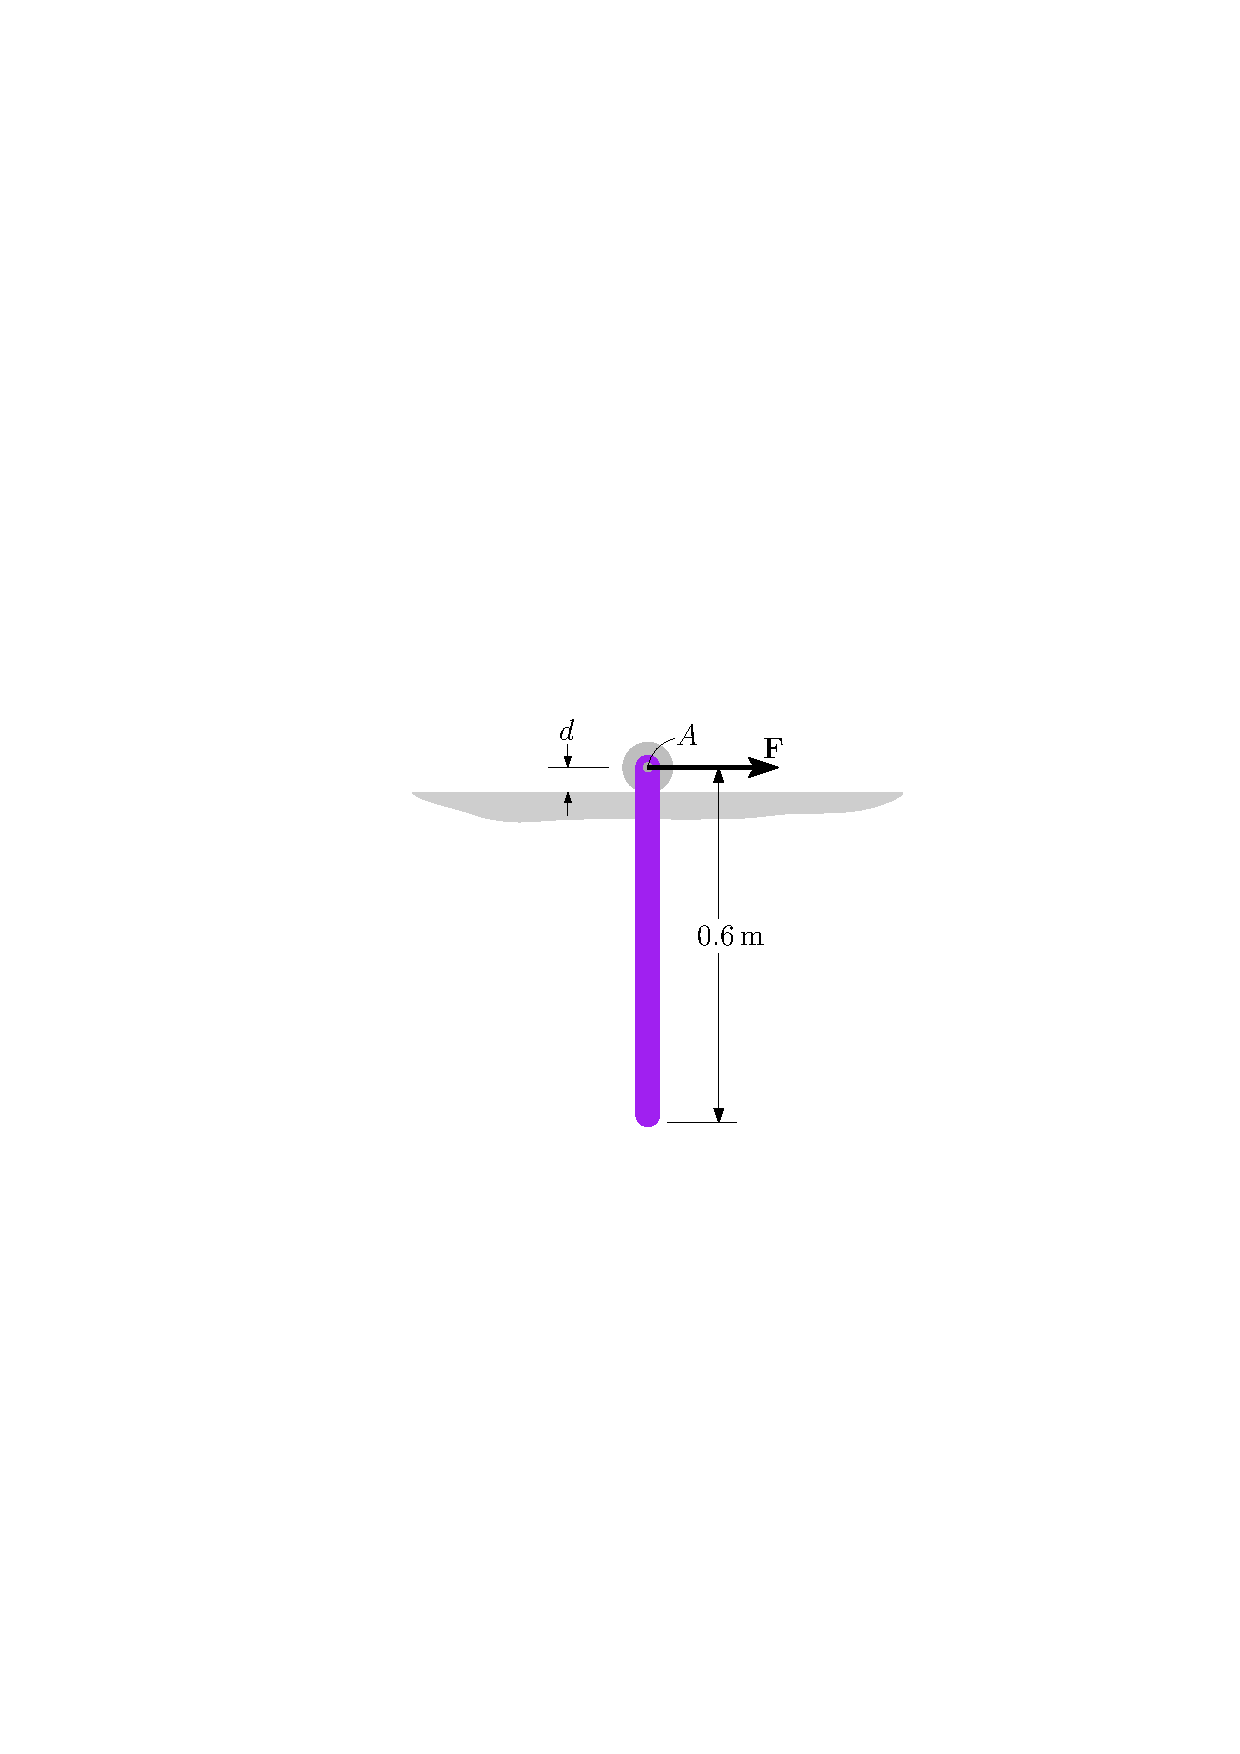
\includegraphics[scale=.9]{../../images/draw_11}
	\end{flushright}
\end{minipage}